\subsection{Задача электрокинетики}

Для примера возьмём систему из \cite{bib:tutor}. Она описывается следующими уравнениями
$$\begin{aligned}
        \vec{j}                                                               & =
        -D \nabla c - \xi z e c \nabla \Phi + c \vec{u}                                    \\
        \partial_{t} c                                                        & =
        -\nabla \cdot\vec{j}                                                               \\
        \nabla^2 \Phi                                                         & =
        -4 \pi l_\mathrm{B} k_\mathrm{B}T z c                                              \\
        \rho \big( \partial_t \vec{u} + (\vec{u} \cdot \nabla ) \vec{u} \big) & =
        -\nabla p_H + \eta \nabla^{2} \vec{u} - (k_\mathrm{B}T \nabla c + zec \nabla \Phi) \\
        \nabla \cdot \vec{u}                                                  & =
        0
    \end{aligned}$$

Здесь первое уравнение в системе описывает поток плотности, второе электростатику, третье гидродинамику с помощью уравнения Навье-Стокса, четвёртое уравнение несжимаемости жидкости.

Рассмотрим систему щелевых пор, состоящую из двух одноимённо заряженных бесконечных пластин. Выпишем для такой системы граничные условия

$$
    \begin{aligned}
        c(t, X_l)       & = 0.01        \\
        c(t, X_r)       & = 0.01        \\
        c(0, X)         & = 0.002       \\
        \vec{v}(t, X_l) & = 0           \\
        \vec{v}(t, X_r) & = 0           \\
        \vec{v}(0, X)   & = 0           \\
        \Phi(t, X_l)    & = -0.05       \\
        \Phi(t, X_r)    & = -0.05       \\
        \Phi(0, X)      & = -0.009x^2+2
    \end{aligned}
$$
здесь $t$ -- время, $X_l$ -- пространственные координаты, соответствующие левой стенке, $X_r$ -- правой, $x$ в формул для $\Phi(0,x)$ соответствует оси, перпендикулярной пластинам.

\subsection{Упрощённый случай}

В начале рассмотрим упрощённую систему уравнений с одной пространственной координатой и без скорости

$$
    \begin{aligned}
        \frac{dc}{dT} & = -\nabla \cdot (- D\nabla c - \xi z e c \nabla \Phi) \\
        \nabla^2 \Phi & = -4 \pi l_\mathrm{B} k_\mathrm{B}T c
    \end{aligned}
$$

С граничными условиями

$$
    \begin{aligned}
        \frac{dc}{dX}(t, 0) & = 0 \\
        \frac{dc}{dX}(t, 1) & = 0 \\
        c(0, X)             & = 1 \\
        \Phi(0)             & = 1 \\
        \Phi(1)             & = 1 \\
    \end{aligned}
$$

Координаты в данном случае нормализованны

$$T = t/t_{\max},\;  X = (x+x_{\min})/x_{\max}$$

где $t_max$ -- время симуляции, $x_max$ -- размер системы по $x$-овой координате, $x_{\min}$ - координата левой стенки. Оператор $\nabla$ действует по пространственным координатам $\nabla = (\frac{d}{d X})$, все константы положим равными 1 и исключим $4\pi$ из второго уравнения.

Запустим обучение следующим образом: 100 запусков обучения (функция \texttt{fit}) по 10 эпох на 10000 наборах точек (внутренняя, граничная и начальная). Обучение заняло 2 минуты 48 секунд, значение функции потерь: $1.7378\cdot 10^{-5}$. Результаты симуляции представлены на рис.~\ref{fig:1d:simp:c} \ref{fig:1d:simp:Fi}:

\begin{figure}[ht]
    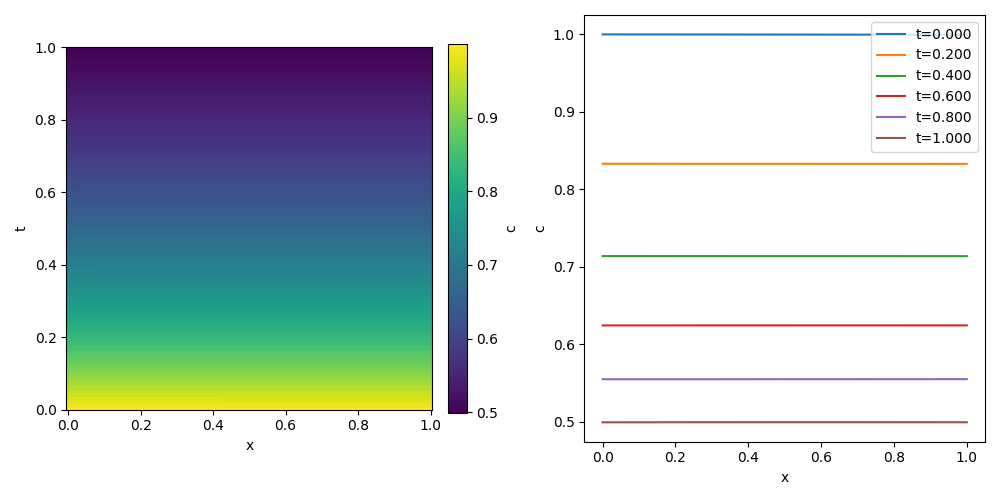
\includegraphics[width=\textwidth]{../plots/1-dim c simpified tanh 80,20.png}
    \caption{Упрощённый случай: концентрация}
    \label{fig:1d:simp:c}
\end{figure}

\begin{figure}[ht]
    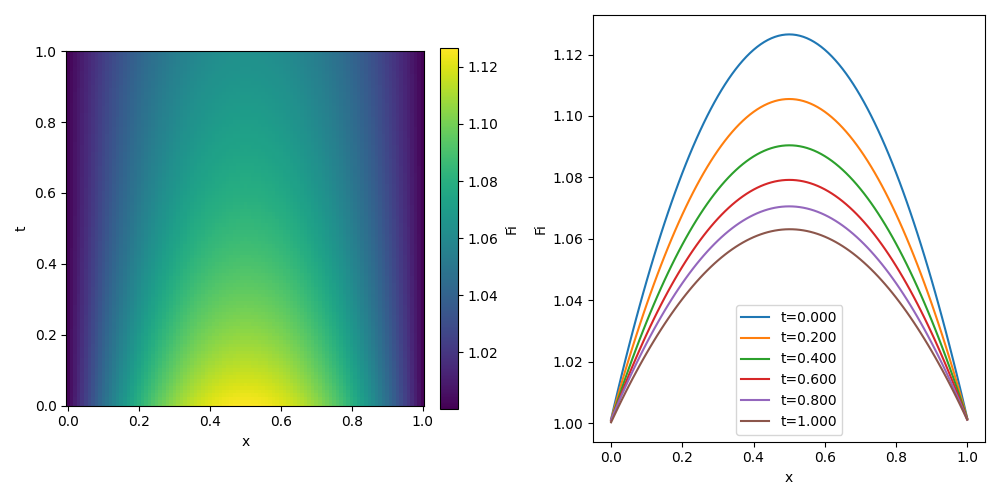
\includegraphics[width=\textwidth]{../plots/1-dim Phi simpified tanh 80,20.png}
    \caption{Упрощённый случай: потенциал}
    \label{fig:1d:simp:Fi}
\end{figure}

\subsection{Полный случай}

Рассмотрим двумерный случай. Скрытые слои будут иметь размеры 80 и 40, входной слой 4, один для концентрации, два для скорости и один для потенциала, функция активации $\tanh$ (гиперболический тангенс). Результат работы после 5000000 итераций показан на графике \ref{fig:2dres}

\begin{figure}[ht]
    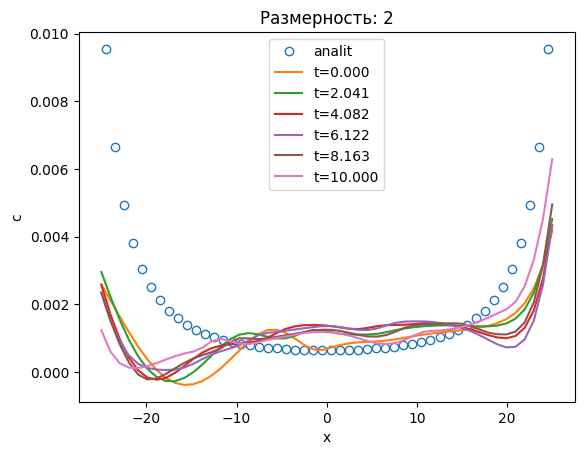
\includegraphics[scale=0.5]{../plots/2dim tanh 80 20.png}
    \caption{}
    \label{fig:2dres}
\end{figure}

Рассмотрим теперь трёхмерный случай. Скрытые слои так же будут иметь размеры 80 и 40, входной слой 5, один для концентрации, три для скорости и один для потенциала, функция активации $relu$. Результат работы после 30000000 итераций показан на графике \ref{fig:3dres}

\begin{figure}[ht]
    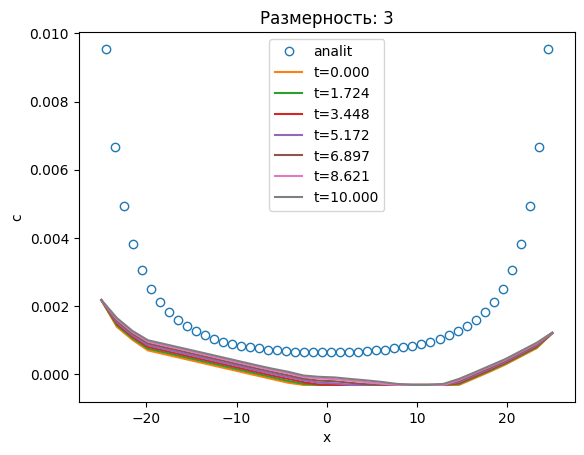
\includegraphics[scale=0.5]{../plots/3dim relu 80 20 30000000.png}
    \caption{}
    \label{fig:3dres}
\end{figure}